\chapter{Konttien orkestrointi\label{orchestration}}

\section{Kontti}

Kontti on karsittu ympäristö, joka koostuu palvelusta ja sen tarvitsemista riippuvuuksista. Kontti tarjoaa vakaan ja suljetun ympäristön palvelun suorittamiselle. Kontti on riippumaton fyysisestä palvelimesta ja sen ulkopuolisestä ympäristöstä, joka mahdollistaa saman kontin toistamisen muilla palvelimilla ja alustoilla. \cite{Jabbari16}

Perinteisistä ja virtuaalikonejulkaisuista poiketen useampi kontti voi käyttää samaa ajoympäristöä ja näin ollen esimerkiksi käyttöjärjestelmän ydintä ei tarvitse säilöä erikseen jokaiseen konttiin. Tämän seurauksena kontit ovat kokonsa ja käynnistysnopeudensa suhteen virtualisointia tehokkaampi ratkaisu. Kuva~\ref{fig:container} esittää resurssien jaon eri julkaisuratkaisuilla. \cite{Dua14}

\begin{figure}[ht]
\begin{center}
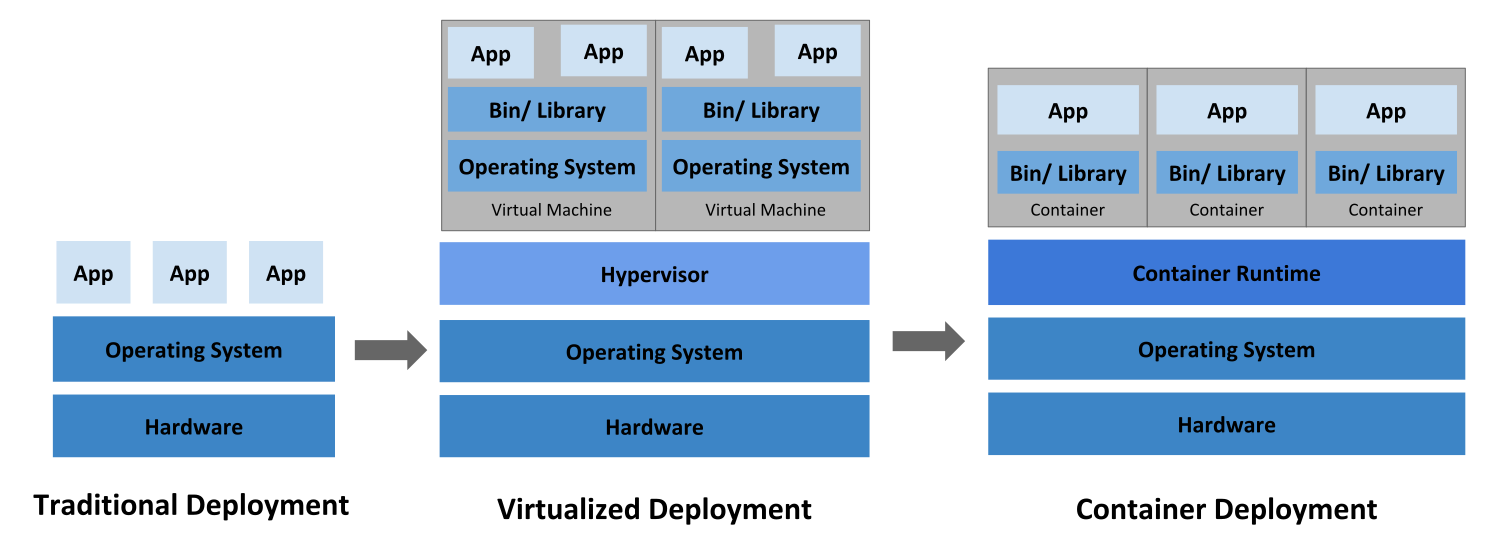
\includegraphics[width=0.9\textwidth]{figures/container_evolution.png}
\caption{Sovelluksen omat ja jaetut resurssit eri julkaisutavoilla.\cite{Kubernetes23}\label{fig:container}}
\end{center}
\end{figure}

\section{Konttien orkestrointi}

Erityisesti mikropalvelupohjaiset järjestelmät saattavat koostu useista sadoista konteista. Myös muun muassa saman palvelun replikaatio ja alueellinen hajauttaminen luovat tarpeen hallinnoida suuria määriä kontteja. \cite{Khan17}

Konttiorkestraatioalustat ovat järjestelmiä, joiden tehtävä on mahdollistaa suurien konttimäärien hallinnointi. Orkestraatioalustat muun muassa hallinnoivat konttien resurssien käyttöä, mahdollistavat konttien monitoroinnin ja huolehtivat konttien virhetilanteista toipumisesta. Kubernetes on laajalti käytetty konttiorkestraatioratkaisu. Se on nykyisistä ratkaisuista suorituskyvyltään tehokkain ja myös toiminnallisuuksiltaan kattavin. \cite{Khan17, Jawarneh19}
